\chapter{脉搏波时域描述特征集的构建及分析处理}
\section{引言}
第三章已经对脉搏波的描述特征参数进行了介绍,本章选取了其中的部分参数构成了基本机器学习的输入数据集。
本章对这部分特征数据按机器学习的一般要求进行了相关处理及准备工作。

\section{脉搏波时域描述特征集的构建}
在第三章基于波形的新型时域特征参数的基础上,本研究选取了其中的部分参数作为后续建立子痫前期识别模型的输入特征集合。出于不同的设计考量,本研究共构建了三个相互独立的脉搏波描述特征集作为
特定模型的训练输入数据。本文的后续分析工作暂未对这三个脉搏波描述特征集进行交叉合并处理。

\subsection{新型时域波形描述特征集合}

如\autoref{fig:road}及\autoref{fig:point}所示,在对脉搏波进行抽象之后,对脉搏波的描述通过选取一系列特殊的基本点$Q$,再借助基于这些选中的基本点的描述指标完成对脉搏波的描述。在使用这种方法对脉搏波进行描述时,
往往需要选取设置多个这样的点,因此,最后的描述结果通常是以向量的形式存在的,即脉搏波波形特征描述向量PPFV。换言之,只要确定了选取基本描述点的原则,就可以得到一系列的基于线段、曲线长度、斜率、弧度及面积等指标的PPFV。
本研究使用了以下原则确定这些基本描述点。

一、左视类指标

左视类指标(Left View Index)是以脉搏波上升支起点为中心,将上升支起点与脉搏波峰值点与水平线的夹角等分成10份。这些等分线与脉搏波的交点即为基本描述点,如\autoref{fig:lv}所示。
\begin{figure}[htbp]
  \centering
  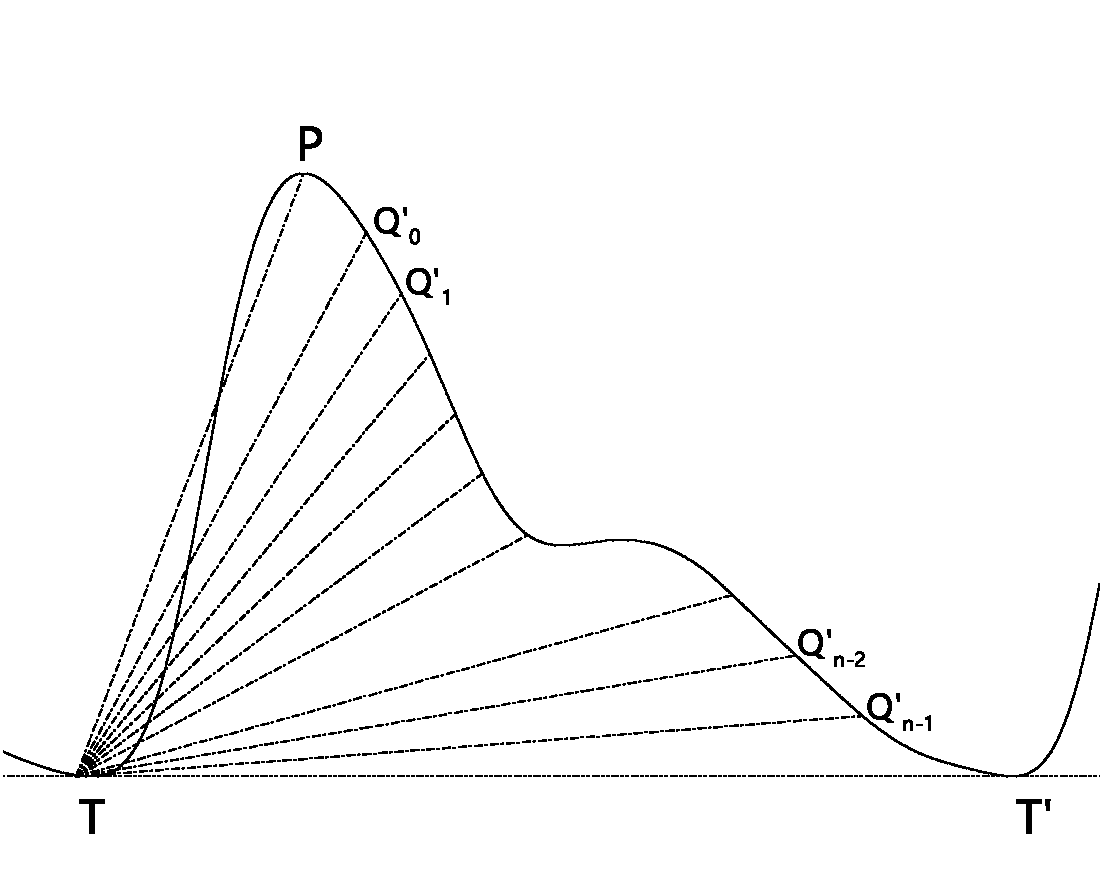
\includegraphics[width=.6\linewidth]{features/lv}
  \caption{\label{fig:lv}左视类指标示意}
\end{figure}

二、中视类指标

中视类指标(Center View Index)是以脉搏波波峰在水平线上的映射点为中心,将上升支与下降支分别等分成10份。这些等分线与脉搏波的交点即为基本描述点,如\autoref{fig:cv}所示。
\begin{figure}[htbp]
  \centering
  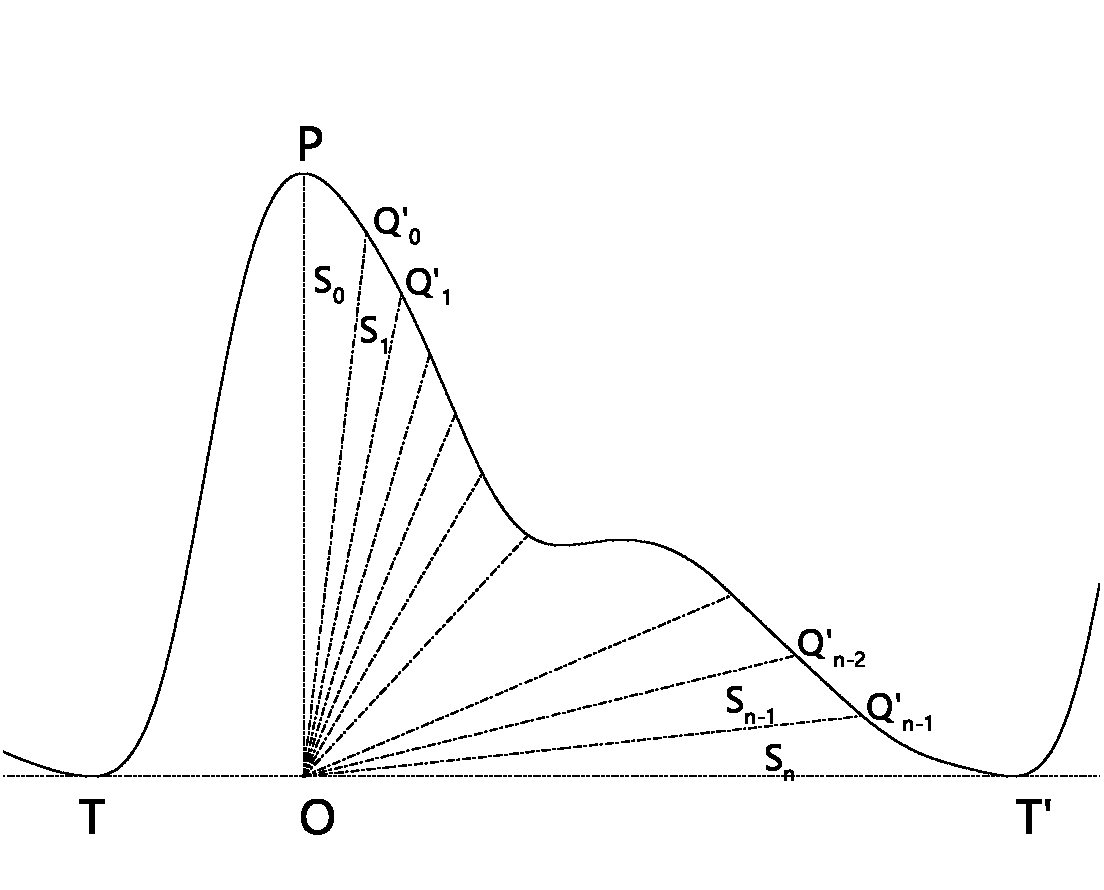
\includegraphics[width=.6\linewidth]{features/cv}
  \caption{\label{fig:lv}中视类指标示意}
\end{figure}

三、分层类指标

分层类指标(Center View Index)是将脉搏波峰值等分为10份后,过各等分点作水平线,取各水平线与上升支与及下降支的交点即为基本描述点,如\autoref{fig:sv}所示。
\begin{figure}[htbp]
  \centering
  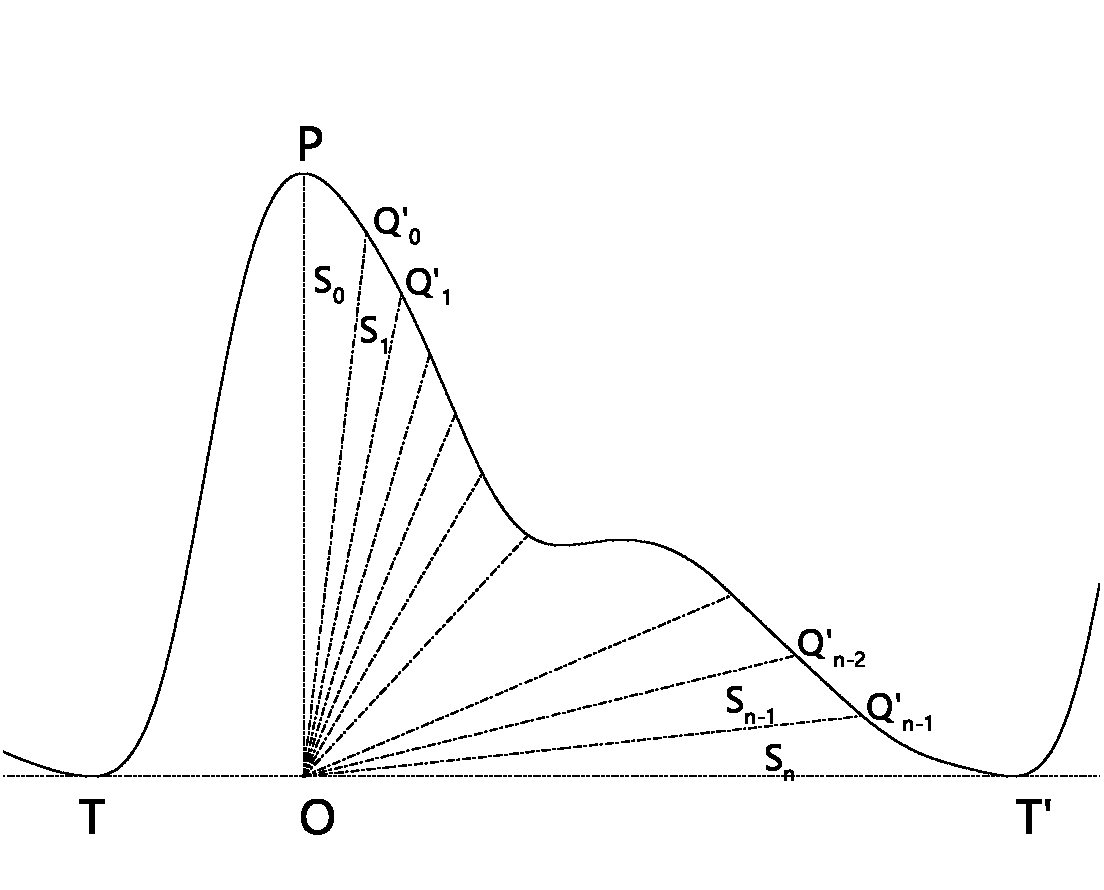
\includegraphics[width=.6\linewidth]{features/cv}
  \caption{\label{fig:sv}分层类指标示意}
\end{figure}

基于以上基本点得到,可以分别得到基于线段、曲线长度、斜率、弧度及面积等指标的PPFV,这些指标如表所示。最后需要指出的是,以上特征参数的计算都是在脉搏波波形标准化之后进行的。
出于方便计算的考虑,所有的脉搏波波形幅值被调整缩放至[0,1000]区间内,其中脉搏波波形上升支与下降支分别进行了线性变换处理。上升支与下降支
在处理时得到的线性变换系数$k$与$b$分别被计为$STD\_RK$、$STD\_RB$、$STD\_RFK$及$STD\_RFB$。
\begin{center}
  \zihao{5}
  \begin{longtable}{m{4cm}<{\centering}m{2cm}<{\centering}m{8.5cm}<{\centering}}
    \caption{本研究使用的所有PPG时域指标一览}\\
    \label{tab:PPGinPE}\\
        \toprule
        \textbf{名称}&\textbf{缩写}&\textbf{意义}\\
        \midrule
        \endfirsthead
        \caption[]{(续)}\\
        \midrule
        \textbf{名称}&\textbf{缩写}&\textbf{意义}\\
        \midrule
        \endhead 
        \midrule
        \endfoot
        \bottomrule
        \endlastfoot
        左视斜率    &   LVS    &   各等分线所对应的直线斜率   \\
        左视上升支交点坐标 & LVLR & 等分线与脉搏波波形上升支交点横坐标 \\
        左视下降支交点坐标 & LVLF & 等分线与脉搏波波形下降支交点横坐标 \\
        左视上升支交点距离 & LVRR & 等分线与脉搏波波形上升支交点与波形起点距离 \\
        左视下降支交点距离 & LVRF & 等分线与脉搏波波形下降支交点与波形起点距离 \\
        左视交点坐标差 & LVD & 左视上升支交点坐标与左视下降支交点坐标之差 \\
        左视上升支弧长 & LVALR & 脉搏波波形上升支被等分线分割的各区间弧长 \\
        左视下降支弧长 & LVALF & 脉搏波波形下降支被等分线分割的各区间弧长 \\
        中视上升支交点坐标 & CVLR & 等分线与脉搏波波形上升支交点横坐标 \\
        中视下降支交点坐标 & CVLF & 等分线与脉搏波波形下降支交点横坐标 \\
        中视上升支交点距离 & CVRR & 等分线与脉搏波波形上升支交点与峰值水平映射点距离 \\
        中视下降支交点距离 & CVRF & 等分线与脉搏波波形下降支交点与峰值水平映射点距离 \\
        中视交点坐标差 & CVD & 中视上升支交点坐标与中视下降支交点坐标之差 \\
        中视上升支弧长 & CVALR & 脉搏波波形上升支被等分线分割的各区间弧长 \\
        中视下降支弧长 & CVALF & 脉搏波波形下降支被等分线分割的各区间弧长 \\
        中视上升支面积 & CVALR & 脉搏波波形上升支被等分线分割的各区域面积 \\
        中视下降支面积 & CVALF & 脉搏波波形下降支被等分线分割的各区域面积 \\
        分层上升支交点坐标 & SVLR & 等分线与脉搏波波形上升支交点横坐标 \\
  \end{longtable}
\end{center}



二、原始波形采样值


三、波形间差异描述特征集合


本小节对本研究实际采用的多种PPG时域描述特征进行汇总,对各参数符号及前置计算条件也进行了统一说明,如\autoref{tab:allfeatures}所示。

\section{脉搏波时域描述特征集的分析处理}
\subsection{数据集的划分}
在大多数机器学习的案例里,将原始数据集重新划分为训练集与测试集是必不可少的一个步骤。

* 分析数据集准备:两种方式

  * A. by pulse

  * B. by person

\subsection{数据清洗}
* 处理缺失值

\subsection{新特征的创建}
* 构建新特征(char参数)
\subsection{特征相关性验证}
* 分布特性

  * 有无差异性,SPSS统计,已用python实现

  * 特征相关性,heatmap
\subsection{特征缩放}
在大多数情况下,原始数据的特征在数值属性出现较大的比例差异会导致机器学习模型的性能下降、表现欠佳\cite{Aurélien2018}。因此,需要对特征数值的分布进行一定的调整使其能够满足具体模型算法的输入要求。
一般的处理原则是同比例缩放所有属性,常见的方法有归一化与标准化两类。

一、归一化

归一化亦称为最小-最大缩放,

二、标准化

balaba
\subsection{特征降维}
事实证明,机器学习模型的训练速度随着训练数据的特征数量增加而降低,这也就是通常而言的维数诅咒或维数灾难。因此,一种可行的策略在构建模型时尽可能只使用“最重要的”特征,即按照特征的贡献度对
原始数据集进行降维处理。但需要注意的是,数据降维在加速训练的同时,通常也会导致系统性能的下降。从这个角度说,特征降维是机器学习过程中的一个可选项而非必选项。

由于特征降维在划分上是数据特征工程的一部分,但在逻辑上的处理又往往与具体的机器学习模型绑定。故本小节暂时只进行概念介绍,真正的降维分析请参见本文后续章节内容。
\section{小结}